\documentclass[11pt]{article}

% ACL 2026 SRW: review mode for submission
\usepackage[review]{acl}

\usepackage{times}
\usepackage{latexsym}
\usepackage[T1]{fontenc}
\usepackage[utf8]{inputenc}
\usepackage{microtype}
\usepackage{inconsolata}
\usepackage{graphicx}
\usepackage{booktabs}

\title{TokLens: A Multilingual Lens on Tokenizer Quality for Large Language Models}

% ACL 2026 SRW: anonymized for double-blind review
\author{Anonymous}

\begin{document}
\maketitle

\begin{abstract}
Tokenizer design is a foundational but underexamined component of large language model (LLM) development. We introduce TokLens, an open-source toolkit for evaluating tokenizer quality across languages using six intrinsic metrics: fertility, characters per token, compression ratio, normalized sequence length, single-token retention rate, and cross-lingual parity. We evaluate 24 tokenizers from major LLM families across 15 typologically diverse languages and correlate intrinsic metrics with downstream performance on the Open LLM Leaderboard v2. Our analysis reveals stark cross-lingual disparities: GPT-2's tokenizer produces 56x more tokens per word in Japanese than in English, while newer tokenizers like Qwen2.5 and Gemma-2 reduce this gap to under 4x. No intrinsic metric predicts English benchmark performance after controlling for model size. However, when we extend the analysis to multilingual benchmarks (MMLU-ProX), tokenizer metrics such as single-token retention rate and characters per token significantly predict per-language performance ($\rho > 0.4$, $p < 0.001$), even after controlling for model size. This suggests that tokenizer quality is a necessary but insufficient condition for strong LLM performance, with its impact most visible in multilingual settings.
\end{abstract}

\section{Introduction}

Subword tokenization is the standard preprocessing step for virtually all modern LLMs \citep{sennrich-etal-2016-neural, kudo-richardson-2018-sentencepiece}. The tokenizer determines how text is segmented into discrete units, directly affecting sequence length, vocabulary coverage, and computational cost. Despite its importance, tokenizer quality is rarely evaluated systematically, particularly across languages.

Recent work has highlighted that tokenizers introduce unfairness between languages \citep{petrov-etal-2024-language, ahia-etal-2023-languages}. Texts in non-Latin scripts are often segmented into many more tokens than equivalent English text, increasing inference cost and degrading effective context length. \citet{rust-etal-2021-good} showed that tokenizer quality correlates with downstream task performance in multilingual masked language models. However, the relationship between tokenizer quality and downstream performance in decoder-only LLMs remains unclear.

As vocabulary sizes have grown from 32K (Llama-2) to 256K (Gemma-2), and training corpora have become more multilingual, the gap between best and worst tokenizers has narrowed, but significant disparities persist. Understanding these disparities, and whether they matter for downstream performance, is important for both model developers and users evaluating multilingual capabilities.

We present TokLens, a lightweight, open-source Python toolkit that computes six tokenizer quality metrics across any number of languages. TokLens is designed to be reusable: researchers can evaluate any HuggingFace-hosted tokenizer on any language with a single command, and model developers can integrate it into their tokenizer development pipeline to audit cross-lingual fairness before deployment (Appendix~\ref{app:toolkit}). Using TokLens, we evaluate 24 tokenizers spanning the major open-weight LLM families and analyze their relationship with downstream benchmarks. Our contributions are:

\begin{enumerate}
    \item An open-source toolkit for systematic tokenizer evaluation with six complementary metrics across 15 languages.
    \item A comprehensive evaluation of 24 tokenizers from 2019--2025, documenting the evolution of multilingual tokenizer quality.
    \item A correlation analysis showing that tokenizer metrics do not predict English benchmarks after controlling for model size, but significantly predict multilingual performance (MMLU-ProX) with partial correlations up to $\rho = 0.48$.
\end{enumerate}

\section{Related Work}

\paragraph{Subword tokenization.} BPE \citep{sennrich-etal-2016-neural} and its variants remain the dominant approach. GPT-2 \citep{radford2019language} popularized byte-level BPE. SentencePiece \citep{kudo-richardson-2018-sentencepiece} introduced language-independent tokenization, adopted by Llama \citep{touvron2023llama} and Mistral \citep{jiang2023mistral}. Recent models like Llama 3 \citep{dubey2024llama3} and Qwen2.5 \citep{yang2024qwen2} use tiktoken-style tokenizers with vocabularies exceeding 128K tokens.

\paragraph{Tokenizer evaluation.} \citet{rust-etal-2021-good} introduced fertility as a tokenizer quality metric, finding that it correlates with downstream performance in multilingual masked language models. \citet{petrov-etal-2024-language} formalized tokenizer unfairness across languages. \citet{ahia-etal-2023-languages} quantified the economic impact, finding that API costs for non-English languages can be 2--15x higher. \citet{ali2024tokenizer} found that tokenizer choice has a negligible effect on downstream English performance when training compute is held constant.

\paragraph{Multilingual vocabularies.} \citet{liang-etal-2023-xlm} proposed allocating vocabulary capacity proportionally to each language's corpus size. BLOOM \citep{workshop2023bloom} demonstrated that multilingual vocabulary construction (251K tokens, 46 languages) can achieve near-parity efficiency. Our work evaluates a broader set of 24 tokenizers with six metrics and correlates with the Open LLM Leaderboard v2 reasoning benchmarks.

\section{Metrics}

TokLens computes six metrics on a given tokenizer and text corpus. All metrics operate on token ID sequences with special tokens stripped for fair comparison.

\paragraph{Fertility.} The average number of tokens per whitespace-delimited word. For language $\ell$ with words $w_1, \ldots, w_n$:
\begin{equation}
    \text{Fertility}(\ell) = \frac{1}{n}\sum_{i=1}^{n} |T(w_i)|
\end{equation}
where $T(w_i)$ is the token sequence for word $w_i$. A fertility of 1.0 means every word is a single token; values above 2.0 indicate heavy fragmentation.

\paragraph{Characters Per Token (CPT).} The ratio $|c| / |t|$ of characters to tokens. Higher CPT means better compression, but CPT can be misleading cross-lingually because a single Chinese character carries more semantic content than a Latin character.

\paragraph{Compression Ratio (CR).} UTF-8 bytes divided by token count: $|b| / |t|$. By measuring bytes rather than characters, CR accounts for multi-byte scripts and provides a fairer cross-lingual comparison than CPT.

\paragraph{Single-Token Retention Rate (STRR).} The fraction of words tokenized as a single token. STRR directly measures vocabulary coverage: an STRR of 0.7 means 70\% of words appear intact in the vocabulary.

\paragraph{Normalized Sequence Length (NSL).} Token count divided by character count: $|t| / |c|$, the inverse of CPT. Values below 1.0 mean the tokenizer compresses the text; values above 1.0 indicate expansion.

\paragraph{Parity Ratio.} The ratio of token counts between a target language and English on parallel text: $\text{Parity}(\ell) = |t_\ell| / |t_\text{en}|$. A value of 1.0 means equal treatment; higher values indicate the tokenizer is less efficient for language $\ell$, directly measuring cross-lingual fairness.

\section{Experimental Setup}

\subsection{Tokenizers}

We evaluate 24 tokenizers from major LLM families (Table~\ref{tab:tokenizers}). Twenty-two have scores on the Open LLM Leaderboard v2 \citep{fourrier2024open}; two (Qwen3-8B, DeepSeek-V3) are included for metric-only analysis. Models range from 0.1B to 35B parameters, vocabulary sizes from 32K to 256K tokens, and span three implementation families: byte-level BPE, SentencePiece BPE, and tiktoken-style BPE.

Several models share tokenizers. Phi-3-mini reuses Llama-2's 32K vocabulary. The Qwen2.5 family uses the same 152K tokenizer across all sizes (0.5B to 14B), providing a natural experiment for isolating model size effects.

\begin{table}[t]
\centering
\small
\begin{tabular}{lrrl}
\toprule
\textbf{Tokenizer} & \textbf{Vocab} & \textbf{Params} & \textbf{Type} \\
\midrule
GPT-2 & 50K & 0.1B & BPE \\
Llama-2-7B & 32K & 6.7B & SP-BPE \\
Llama-3.1-8B & 128K & 8.0B & tiktoken \\
Qwen2.5-\{0.5--14\}B & 152K & 0.5--14.8B & BPE \\
Gemma-2-9B & 256K & 9.0B & SP-BPE \\
Mistral-7B-v0.3 & 33K & 7.2B & SP-BPE \\
Mistral-Nemo-12B & 131K & 11.6B & tiktoken \\
Phi-3-mini & 32K & 3.8B & SP-BPE \\
Phi-4 & 100K & 14.7B & tiktoken \\
Yi-1.5-9B & 64K & 8.8B & BPE \\
Falcon-7B & 65K & 7.0B & BPE \\
BLOOM-7B & 251K & 7.1B & BPE \\
Command-R-35B & 255K & 35.0B & BPE \\
StableLM-2-12B & 100K & 12.1B & BPE \\
GLM-4-9B & 151K & 9.0B & tiktoken \\
OLMo-2-7B & 100K & 7.3B & BPE \\
InternLM2.5-7B & 93K & 7.7B & SP-BPE \\
SmolLM2-1.7B & 49K & 1.7B & BPE \\
\midrule
Qwen3-8B & 152K & -- & BPE \\
DeepSeek-V3 & 129K & -- & BPE \\
\bottomrule
\end{tabular}
\caption{Tokenizers evaluated. SP-BPE = SentencePiece BPE. The Qwen2.5 family shares a single tokenizer across all sizes. Bottom two are metric-only (no benchmark scores).}
\label{tab:tokenizers}
\end{table}

\subsection{Languages and Corpora}

We evaluate on 15 languages spanning 6 scripts: English, Chinese, Japanese, Arabic, Hindi, German, Turkish, Korean, Thai, Russian, French, Spanish, Portuguese, Vietnamese, and Indonesian. The scripts covered are Latin, CJK, Arabic, Devanagari, Thai, and Cyrillic. Corpora are drawn from Wikipedia (100 articles per language, approximately 50K characters each).

\subsection{Benchmarks and Correlation Method}

We use scores from the Open LLM Leaderboard v2, which evaluates models on six benchmarks: IFEval, BBH, MATH Lvl 5, GPQA, MUSR, and MMLU-PRO (full scores in Appendix~\ref{app:benchmarks}). We compute Spearman rank correlations between each tokenizer metric and each benchmark across the 22 models with leaderboard entries. We also compute partial Spearman correlations controlling for model size:
\begin{equation}
    r_{xy \cdot z} = \frac{r_{xy} - r_{xz} \cdot r_{yz}}{\sqrt{(1-r_{xz}^2)(1-r_{yz}^2)}}
\end{equation}
where $z$ is model size in parameters. We apply Bonferroni correction across all 77 metric-benchmark pairs ($\alpha_\text{corrected} = 0.00065$).

\section{Results}

\subsection{Cross-lingual Tokenizer Disparities}

Figure~\ref{fig:parity} shows the parity ratio across all tokenizers and languages. GPT-2's tokenizer produces a parity ratio of 8.8x for Japanese, 6.6x for Chinese, and 14.9x for Russian (the highest in our evaluation, driven by poor Cyrillic coverage). Even Llama-2 (32K vocabulary, 2023) shows 5.7x for Japanese and 4.0x for Chinese. Full parity values are in Appendix~\ref{app:parity}.

\begin{figure*}[t]
    \centering
    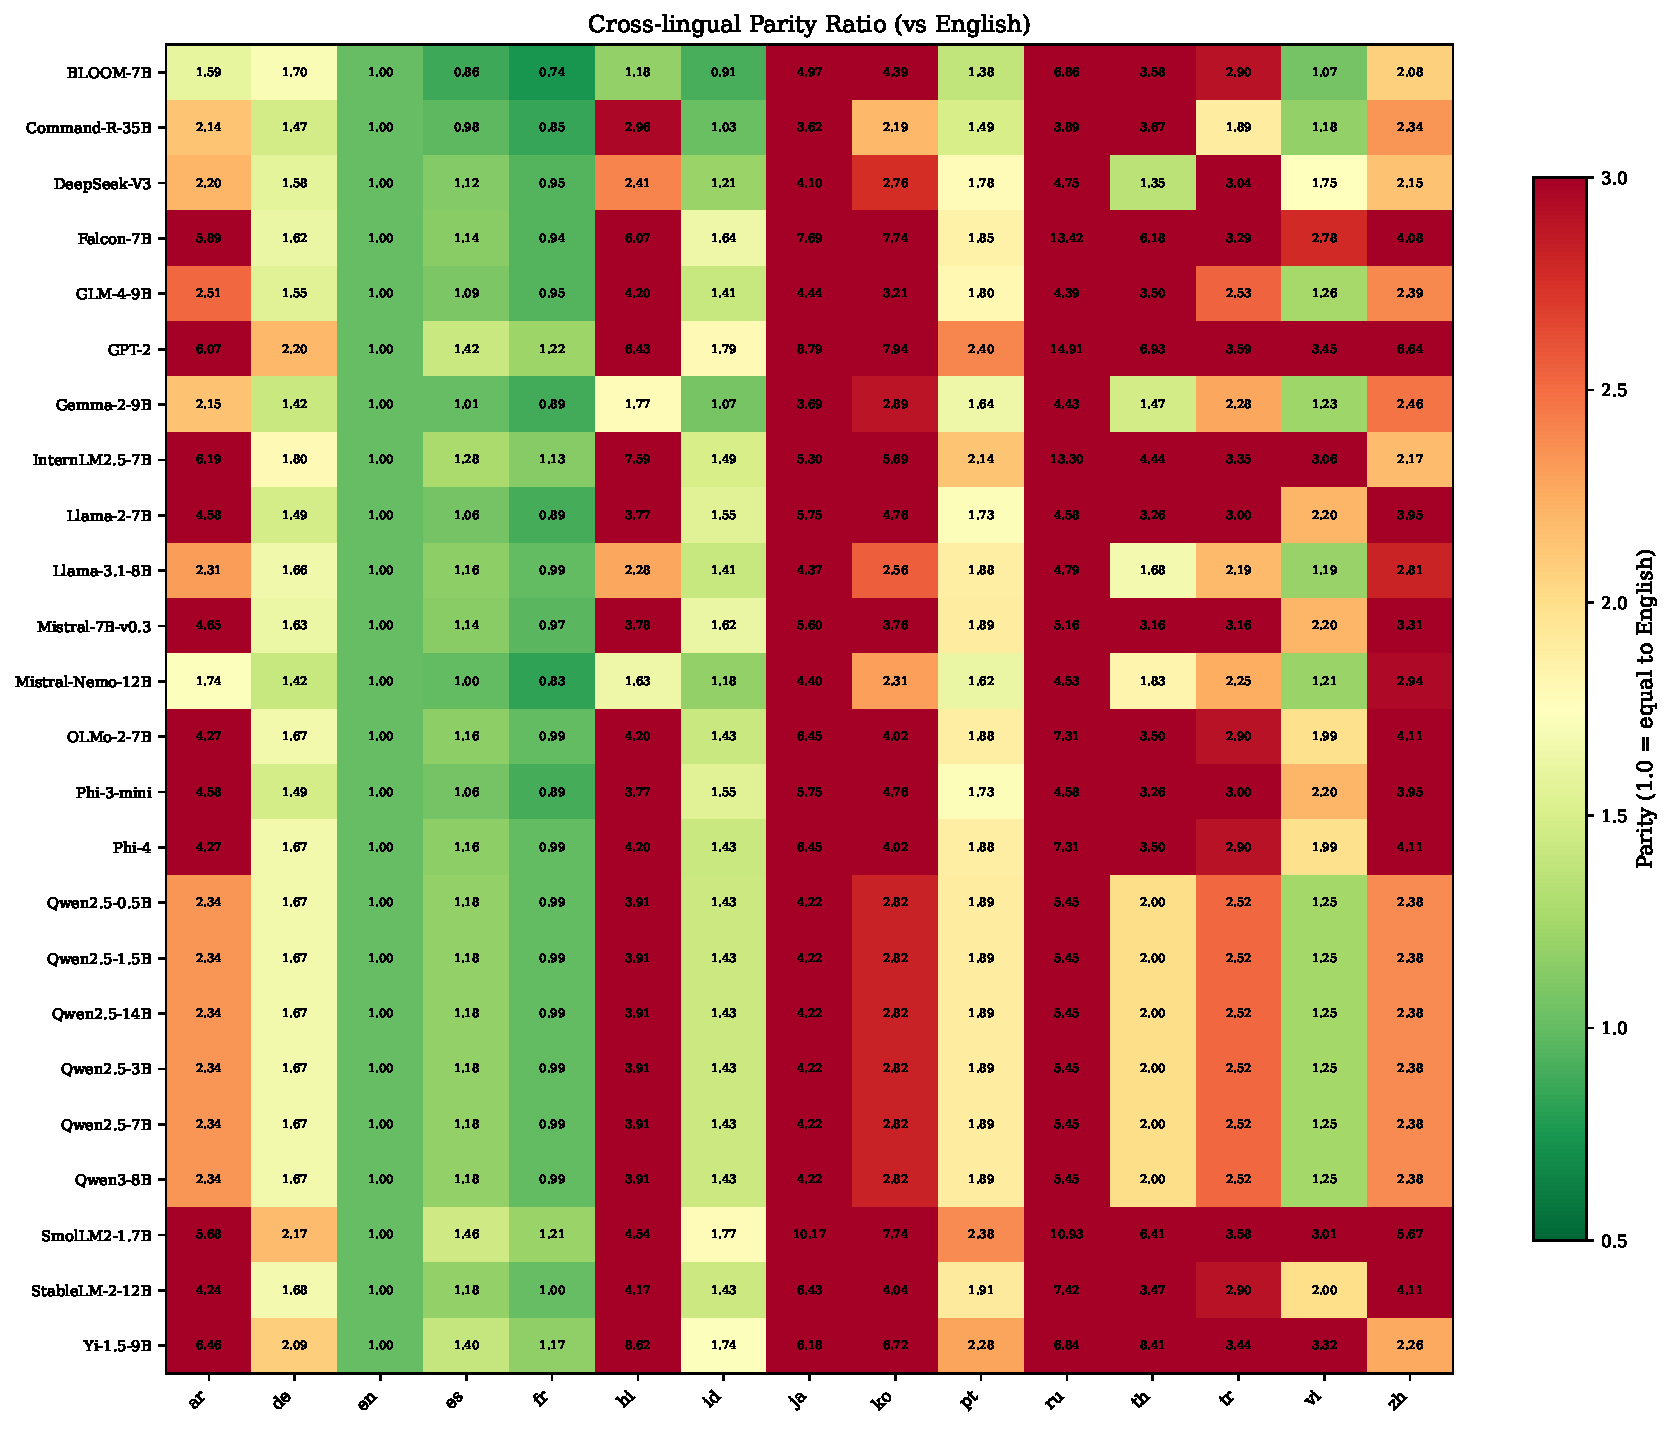
\includegraphics[width=\textwidth]{fig3_parity.pdf}
    \caption{Cross-lingual parity ratio (token count relative to English). Values above 1.0 indicate more tokens are needed than for equivalent English text. Older tokenizers show extreme disparities for CJK, Thai, and Cyrillic, while newer large-vocabulary tokenizers achieve near-parity.}
    \label{fig:parity}
\end{figure*}

In contrast, tokenizers with larger vocabularies and multilingual training data achieve much better parity. BLOOM (251K, explicitly multilingual) reaches parity ratios below 2.0 for most languages. Gemma-2 (256K) and Command-R (255K) show similar improvements. Qwen2.5 (152K), despite a smaller vocabulary, achieves 1.1x parity for Chinese due to its bilingual design, though its Japanese (2.1x) and Korean (2.2x) parity is less impressive.

Among Latin-script languages, parity ratios are generally low (1.0--2.5x) across all tokenizers, since BPE training corpora include substantial Latin-script text. The exceptions are Turkish (up to 3.6x) and Vietnamese (up to 3.5x), which use diacritics that increase byte counts.

\subsection{Fertility and STRR Across Languages}

Figure~\ref{fig:fertility} shows fertility across languages. English fertility ranges from 1.2 (Gemma-2) to 1.6 (GPT-2). For Japanese, the range is dramatic: 91.1 for GPT-2 versus 3.5 for Gemma-2. The extreme GPT-2 values arise from byte-level fallback: Japanese characters require 3 UTF-8 bytes each, so a single character becomes 3 tokens when no vocabulary entry matches.

\begin{figure*}[t]
    \centering
    
\includegraphics[width=\textwidth]{fig4_fertility_by_lang.pdf}
    \caption{Fertility (tokens per word) across 24 tokenizers and 15 languages. CJK languages and Thai show the largest variation. Newer tokenizers with larger vocabularies dramatically reduce fertility for non-Latin scripts.}
    \label{fig:fertility}
\end{figure*}

Korean is an interesting case: it uses a phonetic alphabet (Hangul) with compositional syllable blocks. Tokenizers with good Unicode handling (Qwen2.5, Gemma-2) achieve fertility of 2--4, while byte-fallback tokenizers (GPT-2, Falcon) produce 8--9 because each Hangul syllable is 3 UTF-8 bytes.

Thai presents a different challenge: it does not use spaces between words, so whitespace-delimited ``words'' in Thai text are often entire phrases. This makes absolute fertility values less comparable to other languages, but relative comparisons across tokenizers remain informative. GPT-2 produces a fertility of 53.9 on Thai, while Gemma-2 achieves 4.2, a 13x improvement driven by the inclusion of Thai character sequences in the vocabulary.

For STRR, English ranges from 0.55 (GPT-2) to 0.77 (Gemma-2), meaning that even the best tokenizer splits nearly a quarter of English words into subword pieces. Arabic STRR drops below 0.01 for most tokenizers, reflecting both Arabic's rich morphology (where common words include prefixed articles, prepositions, and pronominal suffixes) and limited vocabulary allocation to Arabic script. Vietnamese, despite using Latin script, has low STRR (0.07--0.20) due to diacritics creating character combinations rarely seen in English-centric training corpora. The full STRR heatmap is in Appendix~\ref{app:strr}.

\subsection{Characters Per Token}

Figure~\ref{fig:cpt} shows CPT across languages. For English, CPT ranges from 4.3 (Llama-2) to 7.0 (Gemma-2). For Chinese, CPT is below 1.0 for most tokenizers, meaning each character produces more than one token on average. The exceptions are BLOOM (2.6), Qwen2.5 (2.8), and Gemma-2 (2.2), which have sufficient CJK vocabulary to compress multiple characters into single tokens. The difference between CPT and compression ratio (CR) is most visible for CJK and Thai: since Chinese characters use 3 UTF-8 bytes each, a CPT of 0.6 (GPT-2 on Chinese) corresponds to a CR of 1.5, revealing that the tokenizer does compress bytes even though it expands characters.

\begin{figure*}[t]
    \centering
    
\includegraphics[width=\textwidth]{fig6_cpt_by_lang.pdf}
    \caption{Characters per token across tokenizers and languages. Higher values indicate more compact tokenization. English consistently has the highest CPT; Chinese and Thai have the lowest for tokenizers without dedicated CJK vocabulary.}
    \label{fig:cpt}
\end{figure*}

\subsection{Correlation with Downstream Performance}

Figure~\ref{fig:heatmap} shows the Spearman correlation heatmap between English tokenizer metrics and benchmarks. Table~\ref{tab:correlations} lists the strongest correlations. The highest absolute correlation is between average fertility and MMLU-PRO ($\rho = -0.38$, $p = 0.08$). However, no correlation reaches significance after Bonferroni correction ($\alpha_\text{corrected} = 0.00065$, 77 comparisons). The full correlation table is in Appendix~\ref{app:correlations}.

\begin{figure*}[t]
    \centering
    
\includegraphics[width=\textwidth]{fig1_heatmap.pdf}
    \caption{Spearman correlation heatmap between English tokenizer metrics and Open LLM Leaderboard v2 benchmarks ($n=22$). No cell reaches significance after Bonferroni correction.}
    \label{fig:heatmap}
\end{figure*}

\begin{table}[t]
\centering
\small
\begin{tabular}{llrrr}
\toprule
\textbf{Metric} & \textbf{Bench} & $\boldsymbol{\rho}$ & $\boldsymbol{p}$ & $\boldsymbol{r_\text{partial}}$ \\
\midrule
Fertility (avg) & MMLU-PRO & $-$0.38 & 0.082 & $-$0.26 \\
CPT (en) & MMLU-PRO & 0.35 & 0.105 & 0.17 \\
Fertility (avg) & MATH & $-$0.35 & 0.111 & $-$0.28 \\
CPT (en) & MUSR & 0.35 & 0.116 & 0.16 \\
NSL (avg) & MMLU-PRO & $-$0.33 & 0.136 & $-$0.10 \\
Parity (avg) & MMLU-PRO & $-$0.32 & 0.141 & $-$0.16 \\
Fertility (avg) & BBH & $-$0.30 & 0.168 & $-$0.16 \\
\bottomrule
\end{tabular}
\caption{Top Spearman correlations between tokenizer metrics and benchmarks ($n=22$). $r_\text{partial}$: partial correlation controlling for model size. No correlation is significant after Bonferroni correction.}
\label{tab:correlations}
\end{table}

Partial correlations controlling for model size are uniformly weaker (Table~\ref{tab:correlations}, rightmost column). The strongest partial correlation is $r = -0.28$ (fertility vs.\ MATH Lvl 5). This suggests the weak raw correlations are partly driven by the confound that larger models tend to have both better tokenizers and higher benchmark scores.

Figure~\ref{fig:scatter} illustrates this confound directly: while there is a visual trend of lower fertility corresponding to higher benchmark scores, the color gradient (model size) reveals that the trend is largely driven by scale. Small models (GPT-2, SmolLM2, Qwen2.5-0.5B) cluster in the lower-right with high fertility and low scores, while large models (Phi-4, Qwen2.5-14B, Command-R) cluster in the upper-left. Within a fixed size range (7--9B), no clear fertility-performance relationship exists.

\begin{figure}[t]
    \centering
    
\includegraphics[width=\columnwidth]{fig2_scatter.pdf}
    \caption{English fertility vs.\ average benchmark score, colored by model size. The apparent negative trend is largely driven by the model size confound: larger models have both better tokenizers and higher scores.}
    \label{fig:scatter}
\end{figure}

Figure~\ref{fig:partial} shows the partial correlation heatmap after removing the model size confound. All values fall within $|r| < 0.3$, with no clear pattern, providing strong evidence that tokenizer metrics carry little predictive power beyond model scale for English benchmarks.

\begin{figure*}[t]
    \centering
    
\includegraphics[width=\textwidth]{fig1b_partial_heatmap.pdf}
    \caption{Partial Spearman correlation controlling for model size. After removing the model size confound, all correlations are weak ($|r| < 0.3$), confirming that tokenizer metrics do not predict English benchmark performance.}
    \label{fig:partial}
\end{figure*}

\subsection{Vocabulary Size and Performance}

Figure~\ref{fig:vocab} plots vocabulary size against average benchmark score. Vocabulary size shows no meaningful correlation with performance. Among 7--9B models, vocabulary sizes range from 32K to 256K, yet scores vary more with architecture and training data.

\begin{figure}[t]
    \centering
    
\includegraphics[width=\columnwidth]{fig7_vocab_vs_benchmark.pdf}
    \caption{Vocabulary size vs.\ average benchmark score, colored by model size. The dominant factor is model scale, not vocabulary size.}
    \label{fig:vocab}
\end{figure}

The Qwen2.5 family provides a natural controlled experiment: all sizes share the same 152K tokenizer, and performance scales cleanly with parameters (0.5B: 6.6, 1.5B: 13.9, 3B: 18.1, 7B: 26.0, 14B: 32.0). BLOOM-7B (251K vocab) scores 3.8, lower than Llama-2-7B (8.8, 32K vocab) and far below Qwen2.5-7B (26.0, 152K vocab), demonstrating that a large vocabulary does not compensate for architecture and training data differences.

\subsection{Multilingual Downstream Correlation}

To test whether tokenizer quality predicts \emph{multilingual} downstream performance, we correlate per-language TokLens metrics with per-language scores from MMLU-ProX \citep{li2025mmluprox}, a multilingual extension of MMLU-Pro with 5-shot chain-of-thought prompting. We identify 7 overlapping models across 11 shared languages, yielding 77 (model, language) data points. For each pair, we compute TokLens metrics in that language and pair them with the corresponding MMLU-ProX score.

Figure~\ref{fig:multilingual} shows the Spearman correlations. In contrast to the English-only null result, several metrics significantly correlate with multilingual performance. Partial correlations controlling for model size are \emph{stronger} than raw: STRR partial $\rho = +0.48$ ($p < 0.001$), CPT $+0.44$ ($p < 0.001$), fertility $-0.36$ ($p = 0.001$). Three survive Bonferroni correction ($\alpha = 0.0083$).

\paragraph{Mixed-effects models.} Since observations from the same model are correlated, we also fit linear mixed-effects models (LME): score $\sim$ z(metric) + log(params) + (1$|$model). LME results confirm the Spearman findings: STRR ($\beta = +5.68$, $z = 18.5$, $p < 0.001$), CPT ($\beta = +5.03$, $z = 11.0$, $p < 0.001$), and parity ($\beta = -4.29$, $z = -7.4$, $p < 0.001$). The model random intercept variance is large (100--115), confirming that model identity is the dominant source of variation, but tokenizer metrics provide significant additional explanatory power. Full LME results are in Appendix~\ref{app:lme}.

\paragraph{Controlled experiment: Qwen2.5 scaling.} The Qwen2.5 family (0.5B--14B) shares the exact same 152K tokenizer, providing a natural controlled experiment where only model size varies. We regress per-language MMLU-ProX scores on log(params) and correlate scaling slopes with TokLens metrics. STRR shows a striking correlation with scaling slope ($\rho = +0.91$, $p < 0.001$; Appendix~\ref{app:qwen}): English (STRR = 0.64) gains 34.9 MMLU-ProX points per decade of scale, while Hindi (STRR = 0.04, a 16x gap) gains only 25.8, nearly 10 points less. Same tokenizer, same architecture, same training pipeline, yet tokenizer quality sets a ceiling on how much each language benefits from scaling.

\begin{figure}[t]
    \centering
    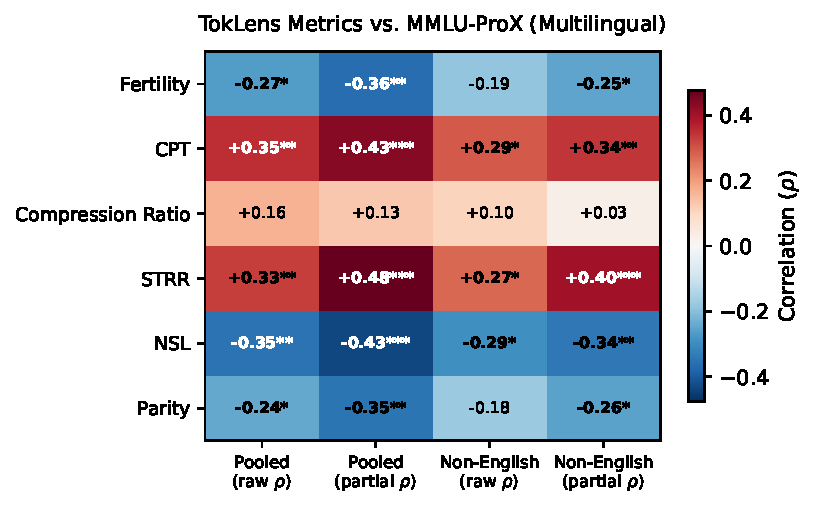
\includegraphics[width=\columnwidth]{fig8_multilingual_corr.pdf}
    \caption{Correlation between TokLens metrics and MMLU-ProX scores across 7 models and 11 languages. Stars: * $p < 0.05$, ** $p < 0.01$, *** $p < 0.001$. Partial correlations control for model size. Unlike English-only analysis, several metrics significantly predict multilingual performance.}
    \label{fig:multilingual}
\end{figure}

\section{Discussion}

\paragraph{Cross-lingual equity has improved but gaps remain.} From GPT-2 to Gemma-2, worst-case parity dropped from 14.9x to under 3x \citep{ahia-etal-2023-languages}. Vocabulary composition matters more than size: Qwen2.5 (152K) achieves better Chinese parity than BLOOM (251K) or Gemma-2 (256K).

\paragraph{Tokenizer quality predicts multilingual but not English performance.} No metric correlates with English benchmarks after controlling for model size, aligning with \citet{ali2024tokenizer}. However, Spearman correlations ($\rho$ up to 0.48), LME models ($z$ up to 18.5), and the Qwen2.5 controlled experiment ($\rho = 0.91$) all confirm that tokenizer metrics predict per-language MMLU-ProX scores. English is well-served by all tokenizers, leaving little room for tokenizer quality to matter. For non-English languages, where quality varies dramatically, the impact becomes measurable.

\paragraph{Practical implications.} A fertility of 91 (GPT-2 on Japanese) means a 4K context window provides only 71 effective words. TokLens enables auditing such disparities for any HuggingFace tokenizer without GPU (Appendix~\ref{app:toolkit}). We recommend vocabularies of at least 100K for cross-lingual parity below 3x, explicitly multilingual training corpora, and routine TokLens-style evaluation.

\section{Conclusion}

We introduced TokLens, an open-source multilingual tokenizer evaluation toolkit, and analyzed 24 tokenizers across 15 languages. No metric predicts English benchmarks, but STRR, CPT, and parity significantly predict multilingual performance (LME $p < 0.001$; Qwen2.5 controlled $\rho = 0.91$). We release TokLens for cross-lingual tokenizer auditing.

% ACL 2026 SRW: Limitations section required, does not count toward page limit
\section*{Limitations}

Our multilingual correlation analysis (Section 5.6) partially addresses the English-only limitation of prior work, but is restricted to 7 models and 11 languages from MMLU-ProX. A broader multilingual evaluation with more models and benchmarks would strengthen these findings.

Second, we do not control for training data composition, which co-varies with tokenizer design. Models with multilingual tokenizers were also trained on multilingual data, making it difficult to isolate the tokenizer's contribution. The controlled experiments of \citet{ali2024tokenizer}, which vary only the tokenizer, provide stronger causal evidence but are limited to a single model architecture.

Third, Wikipedia may not represent all text domains. Code, social media, and scientific text have different token distributions, and tokenizer quality may vary across domains.

Fourth, whitespace-based word segmentation is not well-defined for Chinese, Japanese, and Thai, making fertility and STRR less interpretable for these languages. A morpheme-based segmentation would provide more linguistically meaningful metrics but would require language-specific tools.

Fifth, TokLens evaluates only BPE-family tokenizers, not character-level or byte-level models \citep{clark-etal-2022-canine}.

Finally, the English-only sample size ($n=22$) limits statistical power. The multilingual pooled analysis ($n=77$) partially mitigates this, but within-language correlations ($n=7$) remain underpowered.

% ACL 2026 SRW: Ethics statement (recommended)
\section*{Ethics Statement}

This work evaluates tokenizer quality across languages, relevant to the fairness of language technology. Our finding that tokenizers produce dramatically different token counts across languages has implications for API pricing, context window utilization, and model accessibility. We release TokLens as open source to enable tokenizer fairness audits. No human subjects were involved in this research.

% References
\bibliography{custom}

% ACL 2026 SRW: Appendices start after references, do not count toward page limit
\appendix

\section{Benchmark Scores}
\label{app:benchmarks}

Table~\ref{tab:benchmarks} reports the Open LLM Leaderboard v2 scores used in our correlation analysis. All scores are sourced from the official leaderboard.\footnote{\url{https://huggingface.co/spaces/open-llm-leaderboard/open_llm_leaderboard}}

\begin{table*}[t]
\centering
\small
\begin{tabular}{lrrrrrrrr}
\toprule
\textbf{Model} & \textbf{Params} & \textbf{IFEval} & \textbf{BBH} & \textbf{MATH} & \textbf{GPQA} & \textbf{MUSR} & \textbf{MMLU-PRO} & \textbf{Avg} \\
\midrule
GPT-2 & 0.1B & 17.8 & 2.8 & 0.5 & 1.1 & 13.9 & 1.8 & 6.3 \\
Qwen2.5-0.5B & 0.5B & 16.3 & 7.0 & 3.9 & 0.0 & 2.1 & 10.1 & 6.6 \\
Qwen2.5-1.5B & 1.5B & 26.7 & 16.7 & 9.1 & 4.7 & 5.3 & 20.6 & 13.9 \\
SmolLM2-1.7B & 1.7B & 24.4 & 9.3 & 2.6 & 3.9 & 4.6 & 12.6 & 9.6 \\
Qwen2.5-3B & 3.1B & 26.9 & 24.3 & 14.8 & 6.4 & 11.8 & 24.5 & 18.1 \\
Phi-3-mini & 3.8B & 54.8 & 36.6 & 16.4 & 11.0 & 13.1 & 33.6 & 27.6 \\
Llama-2-7B & 6.7B & 25.2 & 10.4 & 1.7 & 2.2 & 3.8 & 9.6 & 8.8 \\
Falcon-7B & 7.0B & 18.2 & 6.0 & 1.0 & 0.0 & 4.5 & 1.4 & 5.2 \\
BLOOM-7B & 7.1B & 13.2 & 4.0 & 0.5 & 1.9 & 1.9 & 1.2 & 3.8 \\
Mistral-7B-v0.3 & 7.2B & 22.7 & 24.0 & 3.0 & 5.6 & 8.4 & 21.7 & 14.2 \\
OLMo-2-7B & 7.3B & 72.4 & 16.3 & 14.9 & 3.8 & 4.7 & 18.6 & 21.8 \\
Qwen2.5-7B & 7.6B & 33.7 & 35.8 & 25.1 & 10.0 & 14.1 & 37.4 & 26.0 \\
InternLM2.5-7B & 7.7B & 55.4 & 57.0 & 25.3 & 13.0 & 16.3 & 30.9 & 33.0 \\
Llama-3.1-8B & 8.0B & 12.5 & 25.3 & 6.6 & 8.1 & 8.7 & 25.4 & 14.4 \\
Yi-1.5-9B & 8.8B & 29.4 & 30.5 & 11.4 & 17.2 & 12.0 & 32.4 & 22.2 \\
Gemma-2-9B & 9.0B & 20.4 & 34.1 & 13.4 & 10.5 & 14.3 & 34.5 & 21.2 \\
GLM-4-9B & 9.0B & 14.3 & 35.8 & 0.0 & 8.8 & 14.2 & 34.9 & 18.0 \\
Mistral-Nemo-12B & 11.6B & 16.3 & 29.4 & 6.0 & 5.8 & 6.5 & 27.5 & 15.2 \\
StableLM-2-12B & 12.1B & 15.7 & 22.7 & 4.3 & 3.8 & 14.5 & 23.0 & 14.0 \\
Qwen2.5-14B & 14.8B & 36.9 & 45.1 & 29.0 & 17.6 & 15.9 & 47.2 & 32.0 \\
Phi-4 & 14.7B & 5.9 & 52.4 & 31.6 & 20.8 & 23.8 & 47.6 & 30.4 \\
Command-R-35B & 35.0B & 67.5 & 34.6 & 3.5 & 7.6 & 16.1 & 26.3 & 25.9 \\
\bottomrule
\end{tabular}
\caption{Open LLM Leaderboard v2 benchmark scores for all 22 models with leaderboard entries, sorted by parameter count. MATH = MATH Lvl 5. Avg = unweighted average of all six benchmarks.}
\label{tab:benchmarks}
\end{table*}

\section{English Tokenizer Metrics}
\label{app:english}

Table~\ref{tab:english_metrics} reports TokLens metrics computed on English Wikipedia text for all tokenizers with unique vocabularies (Qwen2.5 sizes share a single tokenizer and are listed once).

\begin{table*}[t]
\centering
\small
\begin{tabular}{lrrrrrrr}
\toprule
\textbf{Tokenizer} & \textbf{Vocab Size} & \textbf{Fertility} & \textbf{CPT} & \textbf{CR} & \textbf{STRR} & \textbf{NSL} \\
\midrule
GPT-2 & 50,257 & 1.63 & 5.05 & 5.05 & 0.61 & 0.198 \\
Llama-2-7B & 32,000 & 1.52 & 4.27 & 4.28 & 0.70 & 0.234 \\
Llama-3.1-8B & 128,256 & 1.55 & 5.14 & 5.15 & 0.64 & 0.194 \\
Qwen2.5 & 151,665 & 1.57 & 5.09 & 5.10 & 0.64 & 0.196 \\
Gemma-2-9B & 256,000 & 1.42 & 5.18 & 5.19 & 0.73 & 0.193 \\
Mistral-7B-v0.3 & 32,768 & 1.48 & 4.41 & 4.42 & 0.73 & 0.227 \\
Mistral-Nemo-12B & 131,072 & 1.67 & 4.97 & 4.97 & 0.59 & 0.201 \\
Phi-4 & 100,352 & 1.55 & 5.14 & 5.15 & 0.64 & 0.195 \\
Yi-1.5-9B & 63,992 & 1.67 & 4.72 & 4.72 & 0.60 & 0.212 \\
Falcon-7B & 65,024 & 1.61 & 4.86 & 4.86 & 0.62 & 0.206 \\
BLOOM-7B & 250,680 & 1.62 & 5.01 & 5.01 & 0.59 & 0.200 \\
Command-R-35B & 255,029 & 1.48 & 5.14 & 5.14 & 0.69 & 0.195 \\
StableLM-2-12B & 100,289 & 1.57 & 5.09 & 5.10 & 0.64 & 0.196 \\
GLM-4-9B & 151,329 & 1.55 & 5.14 & 5.15 & 0.64 & 0.194 \\
OLMo-2-7B & 100,278 & 1.55 & 5.14 & 5.15 & 0.64 & 0.195 \\
InternLM2.5-7B & 92,544 & 1.67 & 4.88 & 4.89 & 0.58 & 0.205 \\
SmolLM2-1.7B & 49,152 & 1.57 & 5.01 & 5.02 & 0.64 & 0.199 \\
DeepSeek-V3 & 128,815 & 1.58 & 5.15 & 5.16 & 0.62 & 0.194 \\
Qwen3-8B & 151,669 & 1.57 & 5.09 & 5.10 & 0.64 & 0.196 \\
\bottomrule
\end{tabular}
\caption{TokLens metrics on English Wikipedia for all unique tokenizers. Fertility = tokens per word (lower is better). CPT = characters per token (higher is better). CR = compression ratio in bytes per token (higher is better). STRR = single-token retention rate (higher is better). NSL = normalized sequence length (lower is better).}
\label{tab:english_metrics}
\end{table*}

\section{Cross-lingual Parity}
\label{app:parity}

Table~\ref{tab:parity} reports parity ratios for selected tokenizers across non-Latin languages (parity = token count relative to English). Values closer to 1.0 indicate better cross-lingual equity.

\begin{table*}[t]
\centering
\small
\begin{tabular}{lrrrrrrr}
\toprule
\textbf{Tokenizer} & \textbf{zh} & \textbf{ja} & \textbf{ar} & \textbf{hi} & \textbf{ko} & \textbf{th} & \textbf{ru} \\
\midrule
GPT-2 & 6.6 & 8.8 & 6.1 & 6.4 & 7.9 & 6.9 & 14.9 \\
Llama-2-7B & 4.0 & 5.7 & 4.6 & 3.8 & 4.8 & 3.3 & 4.6 \\
Llama-3.1-8B & 2.8 & 4.4 & 2.3 & 2.3 & 2.6 & 1.7 & 4.8 \\
Qwen2.5 & 2.4 & 4.2 & 2.3 & 3.9 & 2.8 & 2.0 & 5.4 \\
Gemma-2-9B & 2.5 & 3.7 & 2.1 & 1.8 & 2.9 & 1.5 & 4.4 \\
Mistral-7B-v0.3 & 3.3 & 5.6 & 4.7 & 3.8 & 3.8 & 3.2 & 5.2 \\
Mistral-Nemo-12B & 2.9 & 4.4 & 1.7 & 1.6 & 2.3 & 1.8 & 4.5 \\
Yi-1.5-9B & 2.3 & 6.2 & 6.5 & 8.6 & 6.7 & 8.4 & 6.8 \\
Falcon-7B & 4.1 & 7.7 & 5.9 & 6.1 & 7.7 & 6.2 & 13.4 \\
BLOOM-7B & 2.1 & 5.0 & 1.6 & 1.2 & 4.4 & 3.6 & 6.9 \\
Command-R-35B & 2.3 & 3.6 & 2.1 & 3.0 & 2.2 & 3.7 & 3.9 \\
GLM-4-9B & 2.4 & 4.4 & 2.5 & 4.2 & 3.2 & 3.5 & 4.4 \\
InternLM2.5-7B & 2.2 & 5.3 & 6.2 & 7.6 & 5.7 & 4.4 & 13.3 \\
SmolLM2-1.7B & 5.7 & 10.2 & 5.7 & 4.5 & 7.7 & 6.4 & 10.9 \\
DeepSeek-V3 & 2.1 & 4.1 & 2.2 & 2.4 & 2.8 & 1.4 & 4.8 \\
\bottomrule
\end{tabular}
\caption{Cross-lingual parity ratios for non-Latin languages (token count / English token count). Models with shared tokenizers (Phi-3 = Llama-2, Phi-4/OLMo-2/StableLM-2 share similar 100K vocabs, Qwen2.5 family identical) are listed once. Values above 3.0 indicate substantial disadvantage for non-English users.}
\label{tab:parity}
\end{table*}

\section{STRR Heatmap}
\label{app:strr}

Figure~\ref{fig:strr} shows the single-token retention rate across all tokenizers and languages. STRR reveals vocabulary coverage: what proportion of words in each language exist as complete entries in the tokenizer's vocabulary.

\begin{figure*}[t]
    \centering
    
\includegraphics[width=\textwidth]{fig5_strr_by_lang.pdf}
    \caption{Single-Token Retention Rate (STRR) across tokenizers and languages. Higher values indicate more words are kept as single tokens. English and Romance languages have high STRR; Arabic, Hindi, and Thai have extremely low STRR across all tokenizers, reflecting both morphological complexity and vocabulary allocation bias.}
    \label{fig:strr}
\end{figure*}

\section{Full Correlation Results}
\label{app:correlations}

Table~\ref{tab:full_corr} reports all Spearman and partial correlations between TokLens metrics and Open LLM Leaderboard v2 benchmarks, sorted by absolute Spearman $\rho$. Only English-only and cross-lingual average metrics are shown (77 total comparisons). Bonferroni-corrected significance threshold: $\alpha = 0.00065$. No correlation reaches this threshold.

\begin{table*}[t]
\centering
\small
\begin{tabular}{llrrrr}
\toprule
\textbf{Metric} & \textbf{Benchmark} & \textbf{Spearman $\rho$} & \textbf{$p$-value} & \textbf{Partial $r$} & \textbf{Partial $p$} \\
\midrule
Fertility (avg) & MMLU-PRO & $-$0.379 & 0.0820 & $-$0.257 & 0.2600 \\
CPT (en) & MMLU-PRO & 0.355 & 0.1053 & 0.173 & 0.4545 \\
CR (en) & MMLU-PRO & 0.355 & 0.1053 & 0.173 & 0.4545 \\
NSL (en) & MMLU-PRO & $-$0.355 & 0.1053 & $-$0.173 & 0.4545 \\
Fertility (avg) & MATH Lvl 5 & $-$0.350 & 0.1108 & $-$0.282 & 0.2152 \\
CPT (en) & MUSR & 0.345 & 0.1159 & 0.162 & 0.4843 \\
NSL (avg) & MMLU-PRO & $-$0.328 & 0.1364 & $-$0.100 & 0.6659 \\
Parity (avg) & MMLU-PRO & $-$0.324 & 0.1407 & $-$0.160 & 0.4881 \\
Fertility (avg) & BBH & $-$0.305 & 0.1682 & $-$0.156 & 0.4995 \\
Parity (avg) & BBH & $-$0.278 & 0.2096 & $-$0.100 & 0.6674 \\
CPT (avg) & MMLU-PRO & 0.265 & 0.2327 & $-$0.025 & 0.9139 \\
NSL (avg) & BBH & $-$0.263 & 0.2379 & $-$0.013 & 0.9566 \\
Fertility (avg) & GPQA & $-$0.257 & 0.2478 & $-$0.107 & 0.6452 \\
Fertility (en) & MMLU-PRO & $-$0.247 & 0.2675 & $-$0.195 & 0.3977 \\
Fertility (avg) & Average & $-$0.241 & 0.2801 & $-$0.090 & 0.6983 \\
STRR (en) & MMLU-PRO & 0.156 & 0.4871 & 0.164 & 0.4770 \\
STRR (en) & Average & 0.098 & 0.6657 & 0.083 & 0.7194 \\
\bottomrule
\end{tabular}
\caption{Selected Spearman correlations between TokLens metrics and benchmarks ($n=22$, 77 total comparisons). ``avg'' = average across 15 languages; ``en'' = English only. Bonferroni threshold $\alpha = 0.00065$. No correlation is statistically significant. Full results are available in the supplementary material.}
\label{tab:full_corr}
\end{table*}

\section{Toolkit Usage}
\label{app:toolkit}

TokLens is a Python library installable via \texttt{pip install toklens}. It requires Python 3.10+ and depends on the HuggingFace \texttt{tokenizers} library and \texttt{numpy}. The following code demonstrates basic usage:

\begin{verbatim}
from toklens import Analyzer

# Load a tokenizer from HuggingFace
analyzer = Analyzer.from_pretrained(
    "meta-llama/Llama-3.1-8B"
)

# Evaluate on built-in multilingual corpora
report = analyzer.evaluate(
    langs=["en", "zh", "ja", "ar"]
)

# Print results table
report.print_table()

# Evaluate on custom text
metrics = analyzer.evaluate_text(
    text="Your custom text here.",
    ref_text="Reference English text."
)
\end{verbatim}

The toolkit computes all six metrics (fertility, CPT, compression ratio, STRR, NSL, parity) in a single pass. For the parity metric, a reference language (default: English) is required. Corpora are loaded from Wikipedia via HuggingFace \texttt{datasets} and cached locally after first download.

The command-line interface supports quick evaluation:

\begin{verbatim}
# Evaluate a single tokenizer
toklens eval meta-llama/Llama-3.1-8B \
    --langs en zh ja ar

# Compare two tokenizers
toklens compare \
    meta-llama/Llama-2-7b-hf \
    meta-llama/Llama-3.1-8B
\end{verbatim}

\section{LME Results}
\label{app:lme}

Table~\ref{tab:lme} reports the linear mixed-effects model results for all six TokLens metrics. Each model has the form: $\text{score} \sim z(\text{metric}) + \log(\text{params}) + (1 \mid \text{model})$, fitted with REML on 77 observations (7 models, 11 languages). The metric is z-scored so that $\beta$ represents the change in MMLU-ProX score per standard deviation of the metric.

\begin{table}[t]
\centering
\small
\begin{tabular}{lrrrr}
\toprule
\textbf{Metric} & $\boldsymbol{\beta}$ & \textbf{SE} & $\boldsymbol{z}$ & $\boldsymbol{p}$ \\
\midrule
STRR & $+$5.68 & 0.31 & 18.5 & $<$0.001 \\
CPT & $+$5.03 & 0.46 & 11.0 & $<$0.001 \\
NSL & $-$4.96 & 0.52 & $-$9.5 & $<$0.001 \\
Parity & $-$4.29 & 0.58 & $-$7.4 & $<$0.001 \\
CR & $+$2.12 & 0.88 & 2.4 & 0.015 \\
Fertility & $-$1.34 & 0.73 & $-$1.8 & 0.065 \\
\bottomrule
\end{tabular}
\caption{Linear mixed-effects model results. $\beta$: fixed effect of z-scored metric. Model random intercept variance ranges from 100 to 115, confirming that model identity explains most variance. Log(params) is significant ($p < 0.04$) in all models. All metrics except fertility reach significance ($p < 0.05$), with STRR, CPT, NSL, and parity surviving Bonferroni correction.}
\label{tab:lme}
\end{table}

\section{Qwen2.5 Scaling Analysis}
\label{app:qwen}

The Qwen2.5 family (0.5B, 1.5B, 3B, 7B, 14B) shares a single 152K tokenizer, making TokLens metrics identical across sizes. Figure~\ref{fig:qwen_scaling} shows MMLU-ProX scaling curves by language; Figure~\ref{fig:slope_metric} correlates scaling slopes with tokenizer metrics.

\begin{figure}[t]
    \centering
    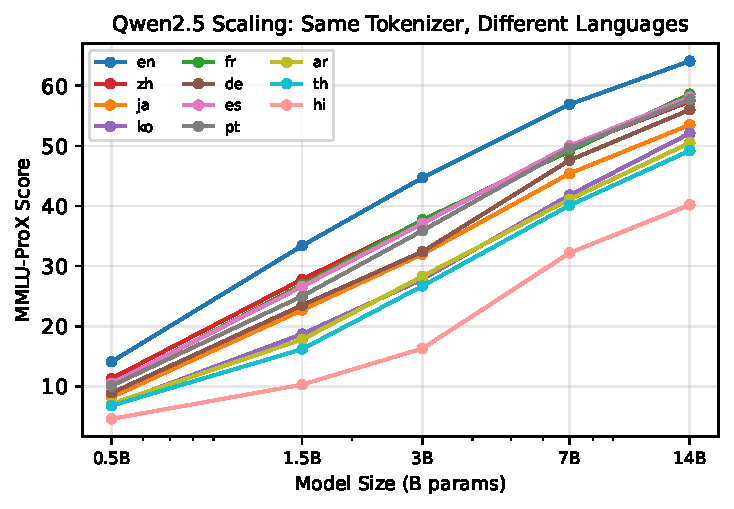
\includegraphics[width=\columnwidth]{fig9_qwen_scaling.pdf}
    \caption{Qwen2.5 MMLU-ProX scaling curves. Each line is a language; all models share the same tokenizer. Languages with better tokenizer quality (en, fr, es) consistently score higher and show steeper scaling.}
    \label{fig:qwen_scaling}
\end{figure}

\begin{figure*}[t]
    \centering
    
\includegraphics[width=\textwidth]{fig10_slope_vs_metric.pdf}
    \caption{Per-language scaling slope (score gain per decade of model size) vs.\ TokLens metrics for Qwen2.5. STRR shows the strongest correlation ($\rho = +0.91$, $p < 0.001$): languages with higher single-token retention benefit more from scaling. Hindi (STRR = 0.04) gains 25.8 points per decade vs.\ 34.9 for English (STRR = 0.64).}
    \label{fig:slope_metric}
\end{figure*}

\end{document}
